\subsubsection{QCD Multijet Reducible Background}
\label{sec:qcdbkg}

The estimation of the contribution from the QCD multijet process in the \etau channel requires two steps. The presence of QCD events in the observed data in the \etau anti-isolated control region biases the previous estimation, as these events are weighted by the inappropriate quark-jet fake rate. Therefore, the first step must be to estimate the yield and \pt distribution of the QCD events in the anti-isolated observed data, in order to correct that bias by subtracting the inappropriate portion of the fake rate estimation. The second step is to perform an independent estimation of the QCD contribution in the signal region using the observed data.

In both steps, a same-sign/opposite-sign (SS/OS) method is used to estimate the number of QCD events in a given region of the data. A same-sign control region is defined by requiring that the light lepton and hadronic tau have the same electric charge, instead of the opposite charge. Because both objects are misidentified jets in QCD events, their charge assignments are expected to be random, so the number of events in which both objects have the same charge should be the same as for the opposite charge. In practice, a slight deviation between the numbers of same-sign and opposite-sign events is possible, for example due to charge asymmetries in proton-proton collisions. The scale factor relating the numbers of same-sign and opposite-sign events was measured to be 1.06 in Ref. \cite{CMS-AN-2013-178}.

The non-QCD background in the same-sign control region is estimated using the simulation and subtracted from the observed data; any remaining events are assumed to originate from the QCD process. The scale factor of 1.06 is applied to extrapolate from this yield $N_{\text{QCD}}^{\text{SS}}$ to the opposite-sign region $N_{\text{QCD}}^{\text{OS}}$:
\begin{align}
N_{\text{QCD}}^{\text{SS}} & = N_{\text{data}}^{\text{SS}} - N_{\text{MC}}^{\text{SS}}, \label{bkg:QCDss}\\
N_{\text{QCD}}^{\text{OS}} & = 1.06 N_{\text{QCD}}^{\text{SS}}. \label{bkg:QCDos}
\end{align}
The subtraction of non-QCD backgrounds can potentially involve a large number of events. In order to ensure the validity of the subtraction, the normalization of the simulated samples must be carefully checked.

To check the normalization of the simulated \W + jets, \Zll, and \Ztt samples, a region of data is defined using the preselection criteria listed in Sec. \ref{sec:presel} without the cut $N_{\text{jets}}\geq2$. Most of the events at the preselection level are eventually eliminated from the signal region by the stricter main and final selections, so the contents of the signal region make up a relatively small portion of this larger region. The transverse mass of the electron and \met system, $\MT(\Pe,\met)$, is defined in Eq. \eqref{eq:MTdef}:
\begin{equation}
\MT(\Pe,\met) = \sqrt{2\pt^{(\Pe)}\met\left[1-\text{cos}\left(\Delta\phi\left(\Pe,\met\right)\right)\right]}. \label{eq:MTdef}
\end{equation}
This definition assumes both particles in the system are massless, which is a good approximation for highly relativistic electrons and neutrinos. The \MT distribution in the region defined above is used to determine normalization parameters for the simulated samples by comparing them to the observed data:
\begin{equation}
\MT^{\text{(data)}} = r_{\W}\MT^{\text{(\W + jets)}} + r_{\tau}\MT^{(\Ztt)} + r_{\ell}\MT^{(\Zll)} + \MT^{\text{(\ttbar,\cPqt,VV)}}. \label{Bkg:eq:MTmin}
\end{equation}
The difference between the sum of the simulated \MT distributions and the observed \MT distribution is minimized by varying the three normalization parameters $r_{\W}$, $r_{\tau}$, and $r_{\ell}$. The normalization of the other processes, \ttbar, single top, and diboson, is not addressed in this minimization. The observed distribution contains a contribution from QCD which is not modeled in the simulation. Therefore, at least one of the normalization parameters will be inflated during the minimization in order to include this contribution. Measurements of the inclusive \W and \Z production cross sections have demonstrated a similarity between the \MT distributions for \Zll and QCD events when using a selection tuned for \Wln events \cite{CMS-AN-2010-359,CMS:2011aa}. Hypothesizing that this similarity holds for the selection considered here, the parameter $r_{\ell}$ should scale the simulated \Zll yield to include the QCD yield.

The minimization in Eq. \eqref{Bkg:eq:MTmin} provides the following values for the $r$ parameters: $r_{W} = 0.86$, $r_{\tau} = 1.21$, $r_{\ell} = 2.02$. Using these parameters, corrected yields $N$ can be defined for the simulated samples, based on the uncorrected yields $N_{\text{MC}}$:
\begin{align}
N(\text{\W + jets}) &= r_{\W}N_{\text{MC}}(\text{\W + jets}), \\
N(\Ztt) &= r_{\tau}N_{\text{MC}}(\text{\Ztt}), \\
N(\Zll) + N(\text{QCD}) &= r_{\ell}N_{\text{MC}}(\text{\Zll}). \label{Bkg:eq:NZllQCD}
\end{align}
Equation \eqref{Bkg:eq:NZllQCD} arises from the hypothesis that the \Zll yield will be scaled to include the QCD yield. This can be used to check the validity of the \MT minimization method for correcting the simulated sample normalizations. The parameter $r_{\tau}$ is assigned to be the normalization correction for both the \Zll and \Ztt samples, in order to solve for $N(\text{QCD})$ in terms of known quantities:
\begin{align}
N(\Zll) &= r_{\tau}N_{\text{MC}}(\text{\Zll}), \label{eq:NZll} \\
N(\text{QCD}) &= r_{\ell}N_{\text{MC}}(\text{\Zll}) - r_{\tau}N_{\text{MC}}(\text{\Zll}). \label{eq:NQCDZ}
\end{align}
Equation \eqref{eq:NQCDZ} follows from the combination of Eqs. \eqref{Bkg:eq:NZllQCD} and \eqref{eq:NZll}. This equation produces the value $N(\text{QCD}) = 24765 \pm 1411$ for the region defined by the preselection criteria without the cut $N_{\text{jets}}\geq2$. In comparison, the SS/OS method applied directly to this region predicts the value $N(\text{QCD}) = 26424 \pm 1250$. These two values agree within uncertainties, validating the assumptions made in the \MT minimization method. The normalization parameters $r_{\W}$ and $r_{\tau}$ will be used for the \W + jets and \Z + jets normalizations in the various same-sign and anti-isolated control regions necessary to conduct the two steps of the QCD estimation in the signal region. A separate control region requiring $N_{\text{b-jet}}\geq2$ and $\MT>70\GeV$ is used to check the normalization of the \ttbar simulation, and no correction is found to be necessary.

To measure the QCD portion of the data in the anti-isolated region, the SS/OS method described by Eqs. \eqref{bkg:QCDss} and \eqref{bkg:QCDos} is applied, using the normalization parameters $r_{W}$ and $r_{\tau}$. Figure \ref{fig:QCDSSAiso} shows the \MT(\Pe,\met) distribution in the same-sign anti-isolated control region for the leptoquark search, with an overall excess in the observed data indicating the presence of QCD. This method predicts $3026\pm210$ QCD events after the leptoquark final selection and $152\pm15$ events after the top squark final selection. In order to subtract these events' contribution from the reducible background estimation, the \pt distribution of the hadronic tau candidates in the QCD events is needed. Figure \ref{Bkg:fig:antiiso} shows that the QCD events in the \etau anti-isolated region are found primarily in the single tau multiplicity bin. Therefore, it is sufficient to subtract the simulated tau \pt distribution from the observed tau \pt distribution to obtain the QCD tau \pt distribution. A simplified version of Eq. \eqref{Bkg:eq:faketauest} can be used to weight these single-tau events:
\begin{equation}
N_{\text{misID}~\tau}^{\text{(QCD)}} = N_{\text{anti-iso}}^{\text{(QCD)}} \sum_{\pt}{\frac{f(\pt)}{1-f(\pt)}}. \label{Bkq:eq:faketausubQCD}
\end{equation}
Using Eq. \eqref{Bkq:eq:faketausubQCD}, the QCD yield to subtract is found to be $38.5\pm2.7$ events in the leptoquark search and $1.5\pm0.1$ events in the top squark search. The subtraction of these QCD yields is already included in the results shown in Tables \ref{Bkg:tab:faketauresultsetauLQ} and \ref{Bkg:tab:faketauresultsetauLQ}, with the statistical uncertainties on the QCD yields included as additional systematic uncertainties on the final major reducible background estimation.

\begin{figure}[hbt]
  \begin{center}
    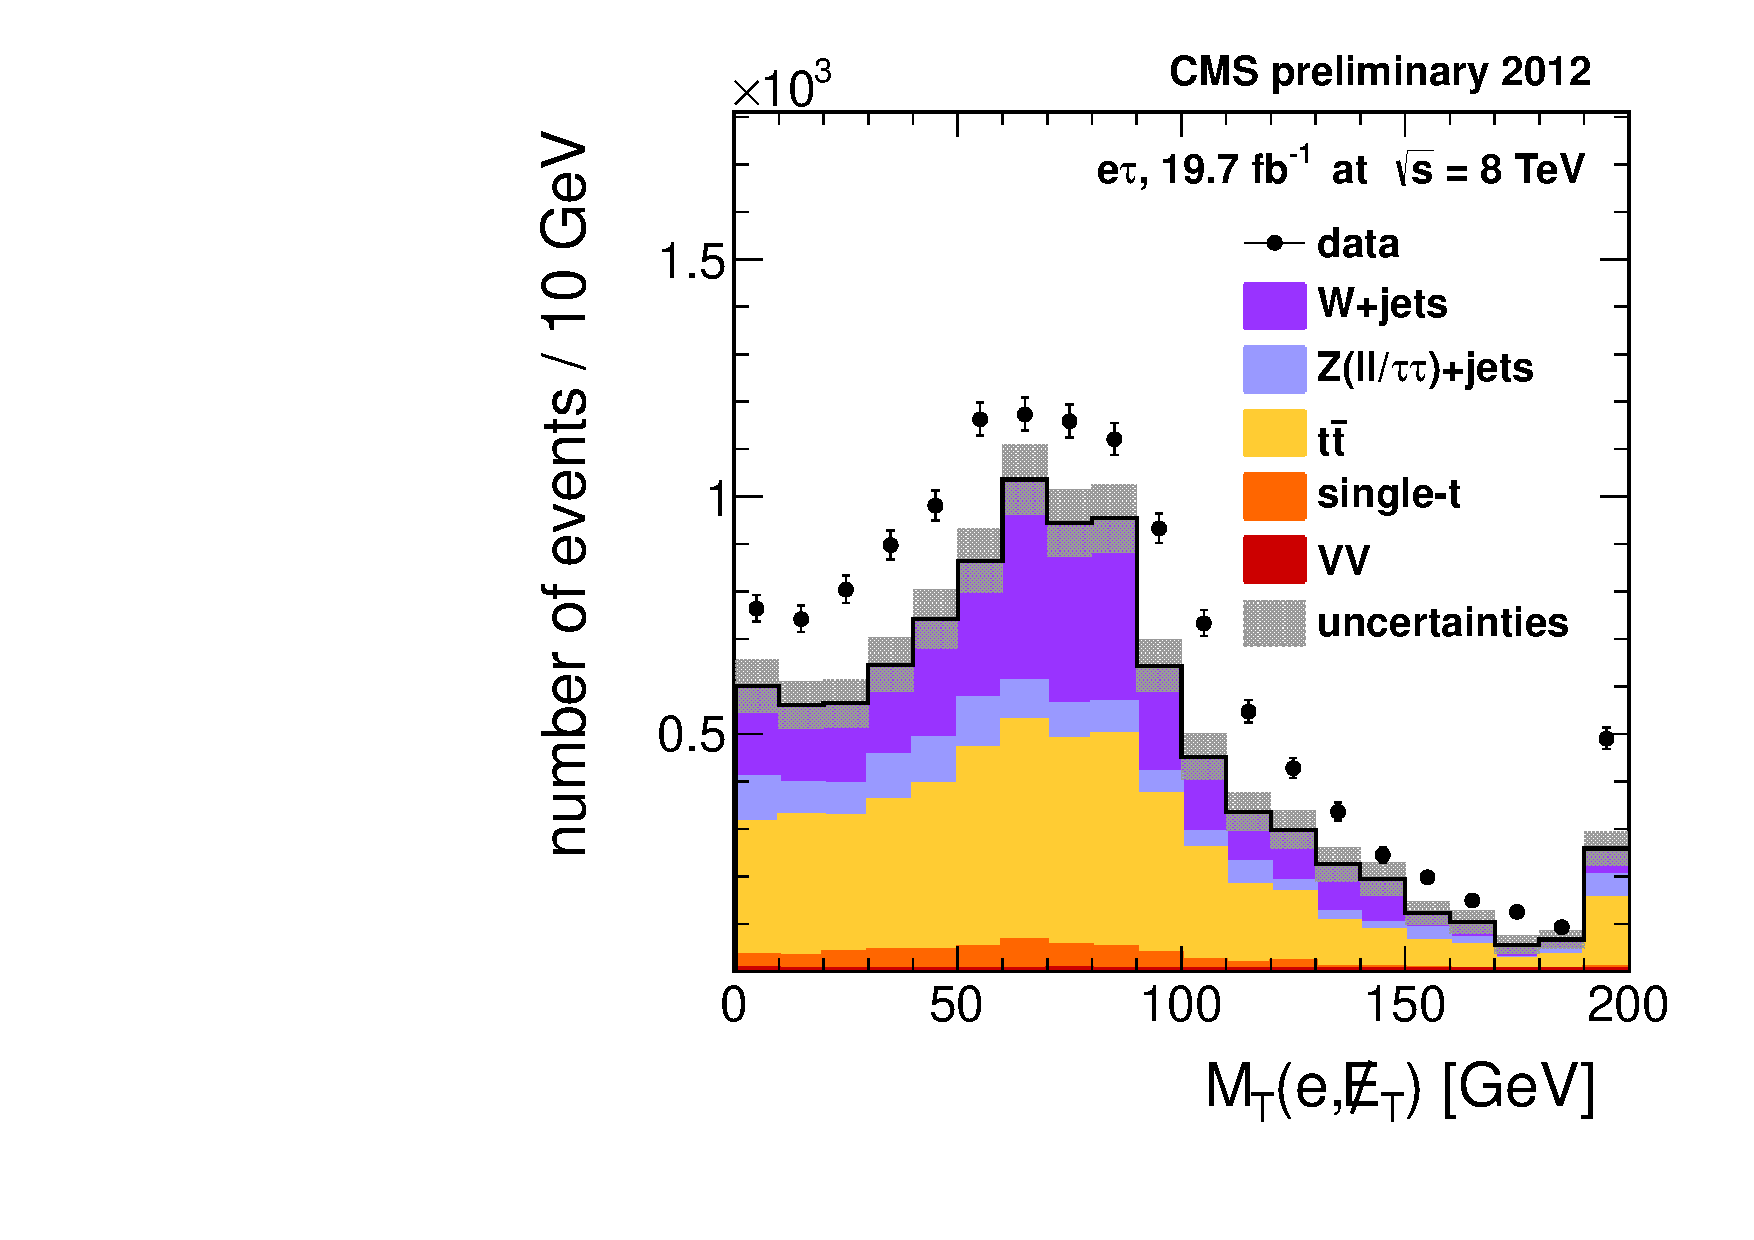
\includegraphics[width=0.6\textwidth]{figures/etau/eMETTMassSSAIsoFinal.pdf}
    \caption{The transverse mass of the electron and missing transverse energy system for the same-sign anti-isolated control region, after the leptoquark final selection. The overall excess in the observed data, not localized in a specific range of \MT values, indicates the presence of QCD events.}
    \label{fig:QCDSSAiso}
  \end{center}
\end{figure}

Having subtracted the improperly estimated QCD contribution, the actual contribution from QCD, if any, must be obtained. Again, the SS/OS method is used, now with the signal region. To decrease the statistical uncertainty in this estimation, the same-sign control region is defined before the final selection. For the leptoquark search, this means that the cut $\MassTJ>250\GeV$ is not applied. Figure \ref{fig:QCDSSMET} shows the \met distribution in this control region, with an excess in the observed data at low \met indicating the presence of QCD. Using the normalization corrections derived previously, the simulated yield in this control region is found to be $474\pm18$ events, while the observed yield is found to be $736\pm27$, which gives $N_{\text{QCD}}^{\text{SS}} = 262\pm32$ and correspondingly $N_{\text{QCD}}^{\text{OS}} = 277\pm34$. To extrapolate this QCD yield to the region defined by the leptoquark final selection, the efficiency of the cut $\MassTJ>250\GeV$ is measured in a same-sign control region which vetoes events containing one or more b-tagged jets, enhancing the contribution from QCD. The QCD yields before and after the mass cut are defined as the subtraction of the simulated yields from the observed yields:
\begin{alignat}{8}
N_{\text{QCD}}^{\text{before}} &= N_{\text{data}}^{\text{before}} &&- N_{\text{MC}}^{\text{before}} &&= (793 &&\pm 28) &&- (469 &&\pm 19) &&= 324 &&\pm 34, \\
N_{\text{QCD}}^{\text{after}} &= N_{\text{data}}^{\text{after}}   &&- N_{\text{MC}}^{\text{after}}  &&= (\hphantom{7}93  &&\pm 10) &&- (\hphantom{4}66  &&\pm \hphantom{1}7)  &&= \hphantom{3}27  &&\pm 12.
\end{alignat}
The ratio of these two yields is the efficiency of the cut, $\varepsilon_{\MassTJ}=8.5\%\pm4.0\%$. Thus, Eq. \eqref{eq:NQCDfinal} calculates the final yield from QCD in the leptoquark search:
\begin{equation}
N_{\text{QCD}}^{\text{final}} = N_{\text{QCD}}^{\text{OS}} \times \varepsilon_{\MassTJ} = (277\pm 34) \times (8.5\% \pm 4\%) = 23.6 \pm 12. \label{eq:NQCDfinal}
\end{equation}
To check this estimation, the SS/OS method is applied to the signal region after the cut $\MassTJ>250\GeV$. This check gives a less precise result $N_{\text{QCD}}^{\text{SS/OS}} = 31.8 \pm 21.2$, which is fully compatible with the above result within uncertainties.

\begin{figure}[hbt]
  \begin{center}
    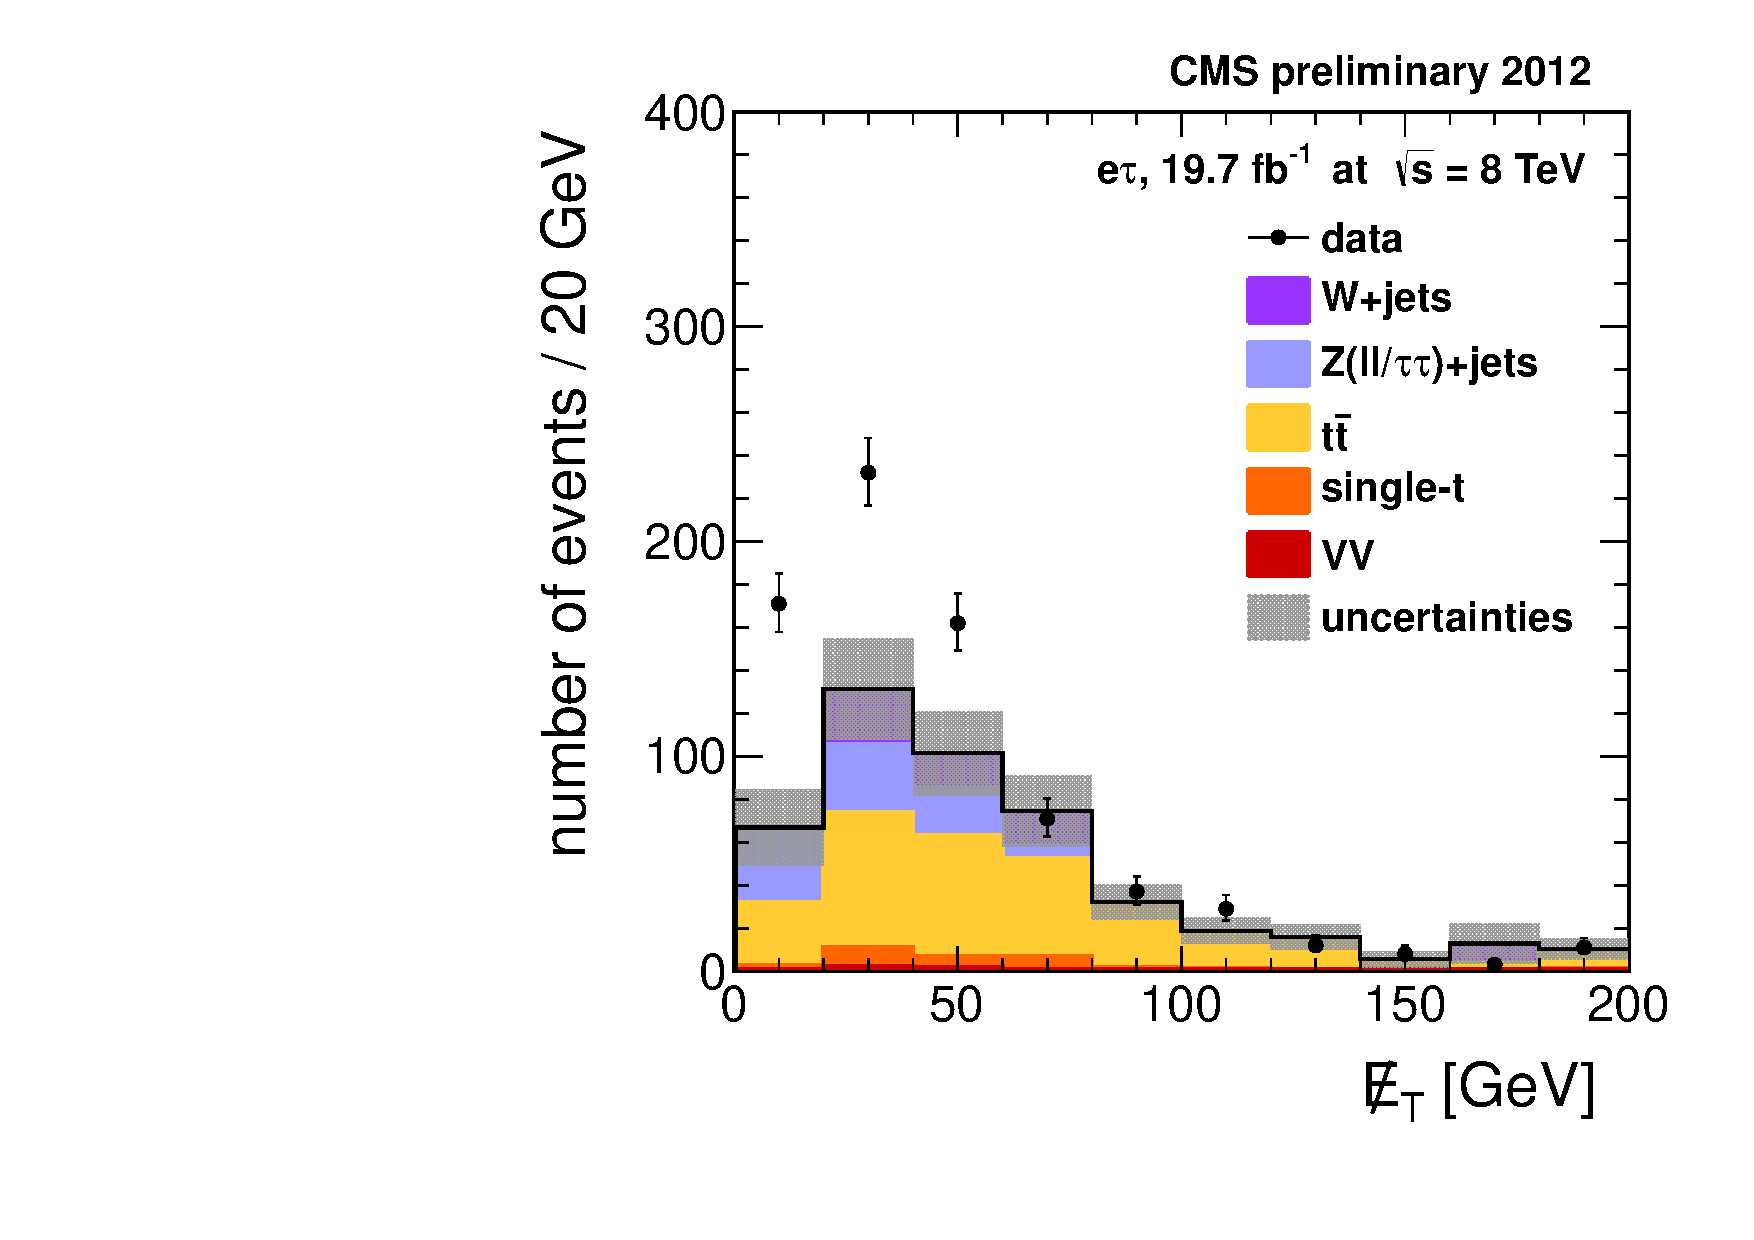
\includegraphics[width=0.6\textwidth]{figures/etau/metPtSSIso.pdf}
    \caption{The missing transverse energy spectrum for the same-sign control region selected before the $\MassTJ>250\GeV$ requirement for the leptoquark search. The excess of observed events at low \met is an indication of the presence of QCD events.}
    \label{fig:QCDSSMET}
  \end{center}
\end{figure}

In addition to the yield, the \ST distribution for the QCD process has to be estimated from the observed data, as no simulated sample is available to produce it. The distribution is obtained by subtracting the simulated \ST distribution of the non-QCD backgrounds from the observed \ST distribution in the same-sign control region after the full leptoquark final selection, as shown in Fig. \ref{fig:residQCD}. The bins with negative values, all of which are equivalent to zero within their statistical uncertainties, are set to be zero to avoid unphysical values in the distribution. The QCD \ST distribution obtained from this method is then added to the major reducible \ST distribution for the \etau channel. The propagated statistical uncertainty on the QCD yield, $\pm 12$ events, is added in quadrature with the systematic uncertainty from the major reducible background estimation.

\begin{figure}[hbt]
  \begin{center}
    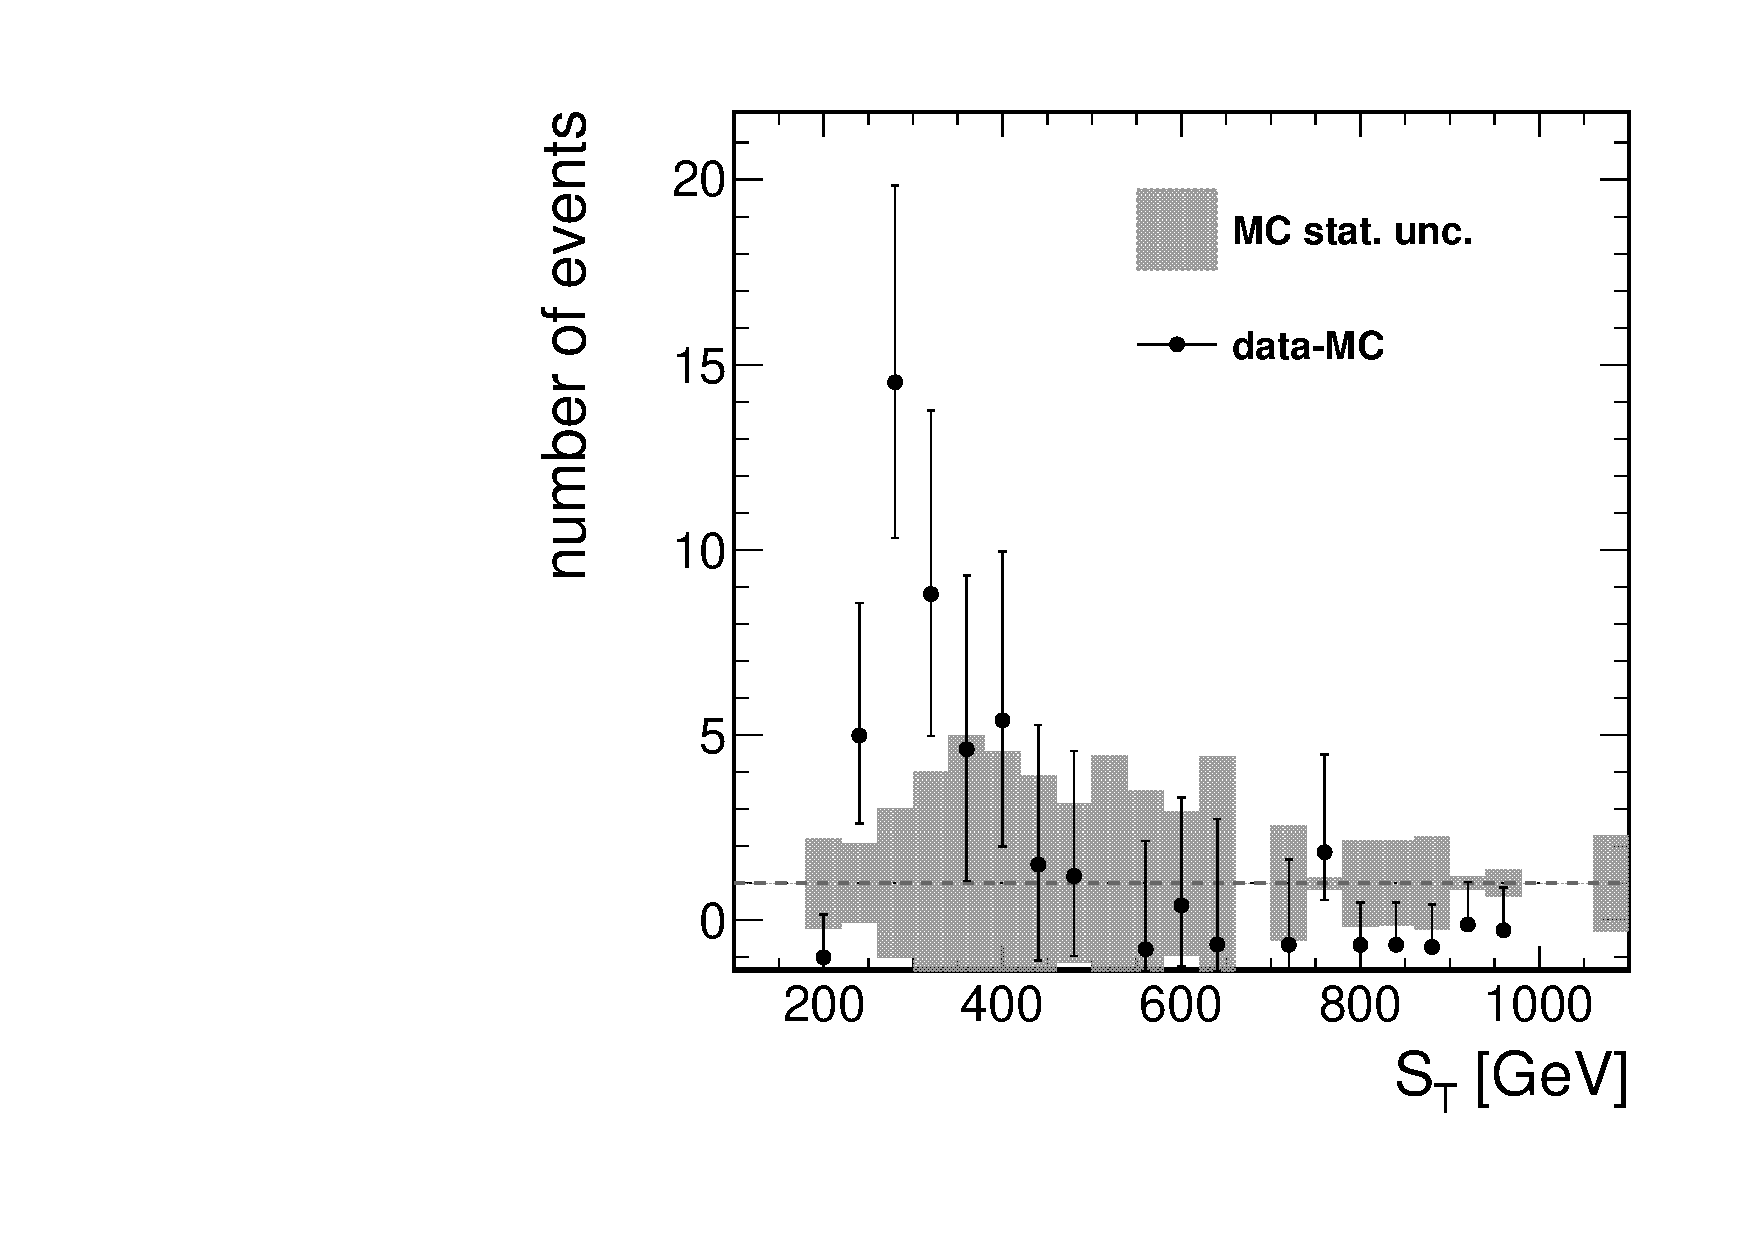
\includegraphics[width=0.6\textwidth]{figures/bkgEstim/residualQCD.pdf}
    \caption{The QCD \ST distribution estimated by subtracting the simulated distribution from the observed distribution in the same-sign control region after the leptoquark final selection. The negative values are set to zero when using the distribution.}
    \label{fig:residQCD}
  \end{center}
\end{figure}

In the top squark search, the QCD background is found to be $0 \pm 13$ using the SS/OS method with an extrapolation of the efficiency of the cut $N_{\text{jets}}\geq5$. Applying the SS/OS method after the final selection to check that prediction finds $0 \pm 18$. These predictions agree and are both equivalent to zero events, so no QCD background is added to the \etau channel in the top squark search. This lack of QCD background is expected due to the high jet multiplicity requirement in this selection.